\documentclass{beamer}

% For more themes, color themes and font themes, see:
% http://deic.uab.es/~iblanes/beamer_gallery/index_by_theme.html
%
\mode<presentation>
{
% Madrid is a good basic theme
%good themes: Antibes/dolphin, Boadilla/beaver/crane

  \usetheme{Antibes}       % or try default, Darmstadt, Warsaw, ... I like Singapore, 
  \usecolortheme{uiowa} % or try albatross, beaver, crane, ... I like seahorse, crane, or beaver
  \usefonttheme{serif}    % or try default, structurebold, ...
  \setbeamertemplate{navigation symbols}{}
  \setbeamertemplate{caption}[numbered]
  \setbeamertemplate{bibliography item}[text]
  %\setbeamercolor{titlelike}{fg=black, bg=white}
} 
\usepackage[english]{babel}
\usepackage[utf8x]{inputenc}
\usepackage{pgfpages}
\pgfpagesuselayout{resize to}[%
  physical paper width=8in, physical paper height=6in]


% Pacakges and commands that I like:
%For math symbols
\usepackage{amsmath} 
\usepackage{amsfonts}%
\usepackage{amssymb}
\usepackage{amsthm}
%\usepackage{titlesec}
%For Graphics
\usepackage{graphicx}
\usepackage{multicol}
\usepackage{subcaption}
%Setup Page
%\usepackage{fullpage} 
% \usepackage[margin=.5in]{geometry}
% \usepackage{fancyhdr}
% \pagestyle{fancy}
% \setlength{\headheight}{14pt}

\def \R{\ensuremath \mathbb{R}}
\def \e{\ensuremath \varepsilon}
\def \d{\ensuremath \delta}
\def \tr{\ensuremath \text{tr}}
\newcommand{\vect}[1]{\boldsymbol{#1}}

\theoremstyle{definition}
\newtheorem{defn}{Definition}[section]
\newtheorem{thm}{Theorem}[section]
\newtheorem*{cor}{Corollary}


% For figures
\newcommand*{\figuretitle}[1]{
  {\centering\scriptsize{
  \textbf{#1}
  \par\medskip}}
}
\newcommand*{\figuretitlesmall}[1]{
  {\centering \tiny{
  \textbf{#1}
  \par\medskip}}
}


%%%%%%%%%%%%%%%%%%%%%%%%%%%%%%%%%%%%%%%%%%%%%%%%%%%%%%%%%%%%%%%%%%%%%%%%%%%%%%
%%%%%%%%%%%%%%%%%%%%%%%%%%%%%%%%%%%%%%%%%%%%%%%%%%%%%%%%%%%%%%%%%%%%%%%%%%%%%%
% Here's where the presentation starts, with the info for the title slide
\title[Neural Network Methods for Application in Educational Measurement]{Neural Network Methods for Application \\ in Educational Measurement}
\author{Geoffrey Converse}
\institute{University of Iowa}
\date{July 15, 2021}

\begin{document}


\begin{frame}
  \titlepage
  \begin{center}
  {\scriptsize PhD Defense in Applied Mathematical and Computational Sciences}
  \end{center}
\end{frame}

\begin{frame}{Overview}
  \begin{itemize}
    \item How can we quantify student learning?
    \item How can we deal with large datasets?
  \end{itemize}
\end{frame}

\begin{frame}{Outline}
  \scriptsize
  \tableofcontents
\end{frame}

\section{Neural Networks}

\begin{frame}{Artificial Neural Networks (ANN)}
\begin{center}
  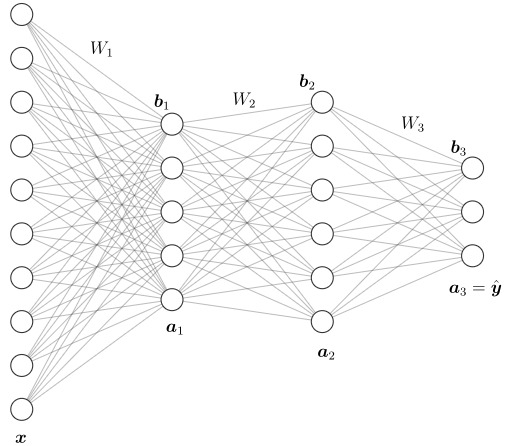
\includegraphics[width=.55\textwidth]{../img/ffn_visual.png}
\end{center}
\scriptsize{Input $\vect x$, approximate a true target $\vect y$ via a series of (learned) linear transformations $W_l$ and nonlinear re-scaling $\sigma(\cdot) : \R^d \to (0,1)^d$}
\[\hat{\vect y} = \sigma(W_3\sigma(W_2\sigma(W_1 \vect x + \vect b_1) + \vect b_2) + \vect b_3)\]
\end{frame}

\subsection{Autoencoders}

\begin{frame}{Autoencoder (AE)}
  \begin{center}
    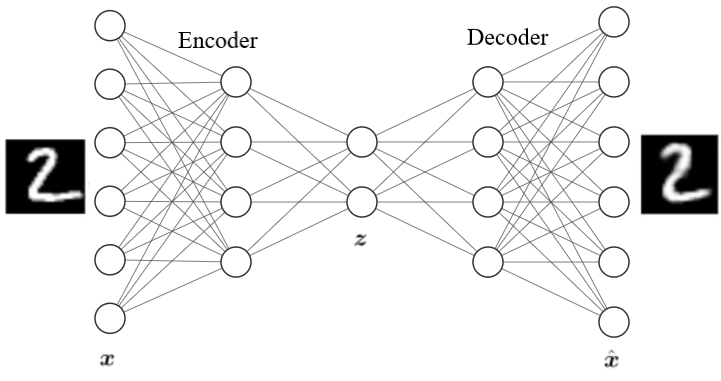
\includegraphics[width=.8\textwidth]{../img/ae_visual.png}
  \end{center}
\begin{itemize}
  \item Encode data into smaller dimension
    \begin{itemize}
      \item Image compression
      \item Non-linear PCA
    \end{itemize}
  \item Reconstruct original input by minimizing $\mathcal{L} = ||\vect x - \hat{\vect x}||$
\end{itemize}
\end{frame}

\subsection{Variational Autoencoders}
\begin{frame}{Variational Autoencoder (VAE)}
\begin{itemize}
  \item Observed data $\vect x$ is generated by some latent code $\vect z$%: $p_x^*(\vect x | \vect z)$
  \item Latent code is assumed to follow a normal distribution $p_z^*(\vect z) = \mathcal{N}(0,I)$
  \item If $\vect z$ is high dimensional, the posterior is intractable:
    \[p_z^*(\vect z | \vect x) = \frac{p_x^*(\vect x | \vect z) p_z^*(\vect z)}{\displaystyle \int p_x^*(\vect x | \vect z) p_z^*(\vect z) d\vect z}\]
  \item Approximate the true posteriors $p_z^*(\vect z | \vect x)$ and $p_x^*(\vect x | \vect z)$ with neural networks $q_\alpha(\vect z | \vect x)$ and $p_\beta(\vect x | \vect z)$

%\item Learn a low-dimensional latent representation $\vect z$ which is capable of generating original data $\vect x$ from some distribution
%\[
%f(\vect z | \vect x)=\frac{P(\vect X=\vect x| \vect z) f(\vect z)}{P(\vect X=\vect x)}
%\]
%\begin{equation}\label{marginal}
%{P(\vect{X}=\vect{x})=\int P(\vect{X}=\vect{x}| \vect{z}) f(\vect{z})d\vect{z}},\nonumber
%\end{equation}
%\item<2-> Approximate $f(\vect{z} | \vect{x})$ with some $q_\alpha(\vect{z} | \vect{x})$ 

\end{itemize}
\end{frame}

%\begin{frame}{Kullback-Leibler Divergence}
%\begin{itemize}
%  \item<1-> \textit{Entropy} measures average information gained from 1 sample:
%  \[H(P) = \mathbb{E}_P[-\log P(x)] =  - \sum_i P(x_i) \log P(x_i)\]
%  \item<2-> \textit{Cross entropy} measures average information needed when using approximate distribution $Q(x)$ instead of true distribution $P(x)$:
%  \[H(P,Q) = \mathbb{E}_P[-\log Q(x)] = -\sum_i P(x_i) \log Q(x_i)\]
%  \item<3-> \textit{Kullback-Leibler Divergence} measures difference between two probability distributions $P(x)$ and $Q(x)$:
%\[\mathcal{D}_{KL} \left[ P(x) || Q(x) \right] = H(P,Q) - H(P) = \sum_i P(x_i) \log \left(\frac{P(x_i)}{Q(x_i)} \right)\]
%%   \item Between an independent, $k$-dimensional, multivariate normal distribution and $\mathcal{N}(0, I)$:
%% \begin{align*}
%% \mathcal{D}_{KL} \left[\mathcal{N}(\mu, \sigma^2) || \mathcal{N}(0, I) \right] = \frac{1}{2} \sum_{i=1}^k (\sigma_i^2 + \mu_i^2 - \ln(\sigma_i^2) - 1)
%% \end{align*}
%\end{itemize}
%\end{frame}

\begin{frame}{VAE Derivation}
  \scriptsize
\begin{equation*}
  \begin{split}
    \log p_x^*(\vect x) &= \int q_\alpha(\vect z |\vect x) \log p_x^*(\vect x)d\vect z \\
    &= \int q_\alpha(\vect z | \vect x) \log \left( \frac{p_z^*(\vect z | \vect x) p_x^*(\vect x)}{p_z^*(\vect z | \vect x)} \right) d\vect z  \\
    &= \int q_\alpha(\vect z | \vect x) \log \left( \frac{p^*(\vect x, \vect z)}{p_z^*(\vect z | \vect x)} \right) d\vect z\\
    &= \int q_\alpha(\vect z | \vect x) \left( \log \frac{q_\alpha(\vect z | \vect x)}{p_z^*(\vect z | \vect x)} + \log \frac{p^*(\vect x, \vect z)}{q_\alpha(\vect z | \vect x)}\right) d\vect z \\
    &= \mathcal{D}_{KL}\left[ q_\alpha(\cdot |\vect x) \big|\big| p_z^*(\cdot | \vect x) \right] + \int q_\alpha(\vect z | \vect x) \log \left( \frac{p^*(\vect x, \vect z)}{q_\alpha(\vect z | \vect x)} \right)d\vect z \\
    &= \mathcal{D}_{KL}\left[ q_\alpha(\cdot |\vect x) \big|\big| p_z^*(\cdot | \vect x) \right] + {\displaystyle\mathbb{E}_{\vect z\sim q_\alpha(\cdot | \vect x)}}\left[ -\log q_\alpha(\vect z | \vect x) + \log p^*(\vect x, \vect z) \right] \\
    &= \mathcal{D}_{KL}\left[ q_\alpha(\cdot |\vect x) \big|\big| p_z^*(\cdot | \vect x) \right] + \tilde{\mathcal{L}}_*(\alpha; \vect x)
\label{eq:vae_derive}
  \end{split}
\end{equation*}

\end{frame}

\begin{frame}{VAE Derivation}
  \scriptsize
  \begin{itemize}
    \item KL-Divergence is non-negative, so we look at the evidence lower bound (ELBO) $\tilde{\mathcal{L}}_*$
  \end{itemize}
  \begin{equation*}
  \begin{split}
    \log p_x^* (\vect x) \geq \tilde{\mathcal{L}}_*(\alpha; \vect x)  &= \mathbb{E}_{\vect z\sim q_\alpha(\cdot | \vect x)}\left[ -\log q_\alpha(\vect z | \vect x) + \log p^*(\vect x, \vect z) \right] \\
    &= \mathbb{E}_{\vect z\sim q_\alpha(\cdot | \vect x)}\left[ -\log q_\alpha(\vect z | \vect x) + \log p_x^*(\vect x | \vect z) + \log p_z^*(\vect z) \right] \\
  &\approx \mathbb{E}_{\vect z\sim q_\alpha(\cdot | \vect x)}\left[ -\log q_\alpha(\vect z | \vect x) + \log p_\beta(\vect x | \vect z) + \log p_z^*(\vect z) \right] \\
  &= -\mathcal{D}_{KL}\left[ q_\alpha(\cdot | \vect x) \big|\big| p_z^*(\cdot) \right] + \mathbb{E}_{\vect z\sim q_\alpha(\cdot | \vect x)}\left[ \log p_\beta(\vect x | \vect z) \right] \\
  &= \tilde{\mathcal{L}}(\alpha, \beta; \vect x)
  \label{eq:elbo}
\end{split}
\end{equation*}

\begin{itemize}
  \item We've replaced all unknown distributions $p_\cdot^*(\cdot)$ with assumed or approximate distributions
  \item VAE loss is given as $\mathcal{L}(\alpha,\beta;\vect x) = - \tilde{\mathcal{L}}(\alpha, \beta; \vect x)$ where $\alpha$ and $\beta$ reference the trainable parameters in the encoder and decoder
\end{itemize}
\end{frame}

\begin{frame}{Variational Autoencoder (VAE)}
\begin{figure}
  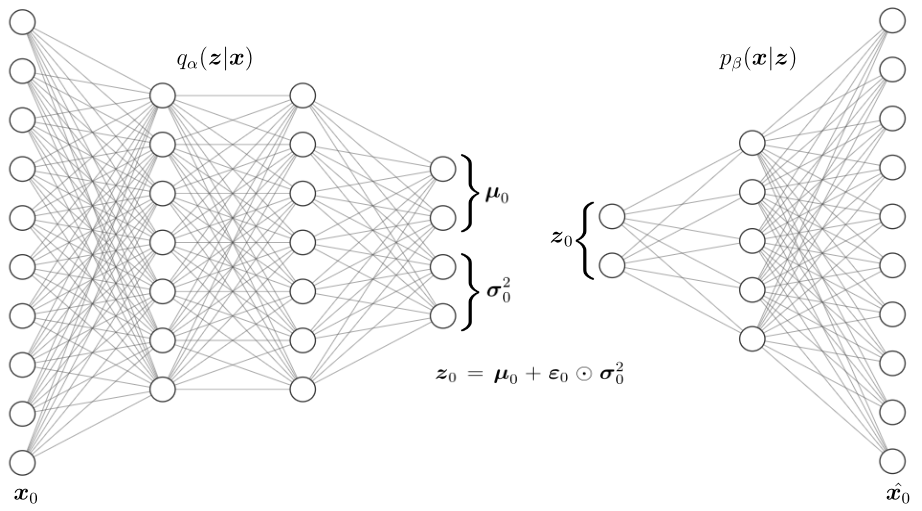
\includegraphics[width=.75\textwidth]{../img/vae_visual.png}
\end{figure}
\scriptsize
\begin{itemize}
  \item<1-> Fit encoded space to $\vect z \sim \mathcal{N}(0,I)$
  \item<1-> Given input $\vect x_0$, the encoder outputs a distribution $q_\alpha(\vect z | \vect x_0) = \mathcal{N}(\vect \mu_0, \vect \sigma_0^2)$
  \item<2-> Sample $\vect \e \sim \mathcal{N}(0,I)$, set $\vect z_0 = \vect \mu_0 + \vect \e \odot \vect \sigma_0$
  \item<2-> Feed $\vect z_0$ through decoder to obtain reconstruction $\hat{\vect x}_0 \sim p_\beta(\cdot | \vect z_0)$
\end{itemize}
\end{frame}

\begin{frame}{Variational Autoencoder (VAE)}
  \scriptsize
  \begin{itemize}
    \item VAE are used as a generative model
    \item Train on a set of images, then generate \textit{new} images which are similar to the training data by sampling form the latent space
  \end{itemize}
  \begin{figure}[h]
    \centering
    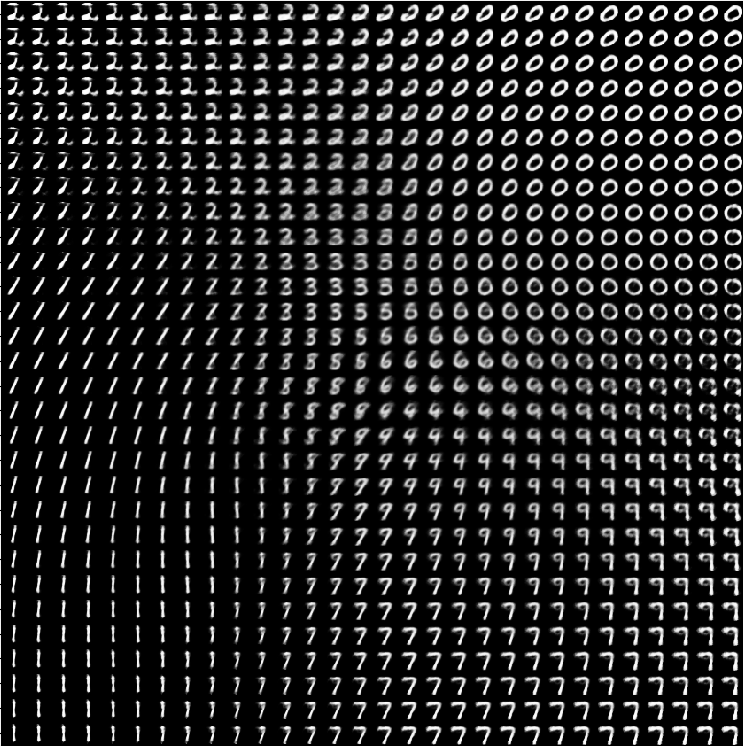
\includegraphics[width=.55\textwidth]{../img/vae_mnist_latent_gen.png}
  \end{figure}
\end{frame}

\section{Item Response Theory}

\begin{frame}{Item Response Theory (IRT)}
  %TODO: clean this up some
\begin{itemize}
  \item Goal: Explain relationship between student ability and exam performance
  \item Each student has a latent ``ability'' value $\theta \in \R$
  \begin{itemize}
    \item<2-> $\theta$ is not directly observable
    \item<2-> Naive solution: $\theta \approx \displaystyle\frac{\text{questions answered correctly}}{\text{total number of questions}}$
  \end{itemize}
  \item<3> For an assessment with $n$ items taken by $N$ subjects, what is the probability that student $j$ answers item $i$ correctly?
  \[P(u_{ij}=1 | \theta_j) = f(\theta_j; \Lambda_i)\]
  \begin{itemize}
    \item<3> $\theta_j =$ latent ability of subject $j$
    \item<3> $\Lambda_i =$ set of parameters for item $i$ (e.g. difficulty)
  \end{itemize}
\end{itemize}
\end{frame}

\begin{frame}{Rasch Model}
\begin{itemize}
  \item Define $\d_i > 0$ as the difficulty of item $i$, and $\eta_j > 0$ the ability of subject $j$.
  \item Rasch: Probability of success depends on ratio $\displaystyle \frac{\d_i}{\eta_j}$
    \[P(u_{ij} = 1 | \eta_j, \d_i) = \frac{1}{1 + \d_i/\eta_j} = \frac{\eta_j}{\eta_j + \d_i}\]
  \item<2-> Logarithmic transformation: $\theta_j = \log \eta_j$ and $\beta_i = \log \d_i$
  \item<2-> Rasch Model:
    \[P(u_{ij} = 1 | \theta_j, \beta_i) = \frac{1}{1 + e^{\beta_i - \theta_j}}\]
\end{itemize}
\end{frame}

\begin{frame}{2-Parameter Logistic Model (2PL)}
\begin{itemize}
  \item Probability of a correct response follows the logistic equation:
    \[P(u_{ij} = 1 | \theta_j; a_i, b_i) = \frac{1}{1 + e^{-a_i(\theta_j - b_i)}}\]
    \item<2-> $a_i =$ discrimination parameter (slope)
      \begin{itemize}
        \item Quantifies the capability of item $i$ in differentiating between students with sufficient/insufficient ability
      \end{itemize}
    \item<2-> $b_i =$ difficulty parameter (intercept)
\end{itemize}
\end{frame}

\begin{frame}{Item Characteristic Curve (ICC)}
\begin{figure}
  \centering
  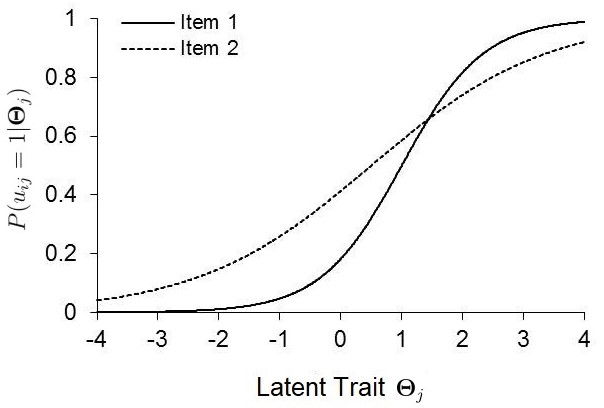
\includegraphics[width=.7\textwidth]{../img/logistic_2param_icc.jpg}
  \begin{itemize}
    \item Item 1 has higher discrimination than Item 2
  \end{itemize}
\end{figure}

\end{frame}
\begin{frame}{Multidimensional IRT}
\begin{itemize}
  \item Now assume that an assessment is testing $K$ skills
  \begin{itemize}
    \item For example, a math exam can test skills add, subtract, multiply, divide
    \item Student $j$ has a vector of skills $\Theta_j = (\theta_{j1},.., \theta_{jK})^T$
    \item Multiple skills can be assessed by a single item
  \end{itemize}
  \item<2-> Binary $Q$-matrix defines relationship between items and skills
  \begin{itemize}
    \item<2-> $Q \in \R^{n \times K}$, \[q_{ik} = \begin{cases}
    1 & \text{if item } i \text{ requires skill } k \\ 
    0 & \text{otherwise} 
    \end{cases}\]
  \end{itemize}
\end{itemize}
\end{frame}

\begin{frame}{Multidimensional Logistic 2-Parameter (ML2P) Model}
\begin{itemize}
\item Probability of correct response given by:
  \begin{align*}
  P(u_{ij}=1 | \Theta_j; \vect a_i, b_i) &= \frac{1}{1+\exp\left[-\vect a_i^\top \Theta_j + b_i\right]} \\
  &= \frac{1}{1 + \exp[-\sum_{k=1}^K q_{ik}a_{ik}\theta_{jk} + b_i]}
\end{align*}
  \begin{itemize}
    \item<2-> $a_{ik} =$ discrimination parameter between item $i$ and skill $k$ 
    \item<2-> $b_i =$ difficulty parameter
  \end{itemize}
\end{itemize}
%TODO: cite daSilva
\end{frame}

\subsection{IRT Parameter Estimation Methods}

\begin{frame}{Estimating IRT Parameters}
  \begin{itemize}
    \item In application, given only binary matrix of $N$ response sets $U \in \R^{N\times n}$
      \begin{itemize}
        \item $\vect u_j \in \R^n$ details student $j$'s correct/incorrect responses to $n$ items
      \end{itemize}
    \item How to obtain the item parameters $\vect a_i$ and $b_i$ and student ability parameters $\vect \Theta_j$?
    \item Maximize the log-likelihood of the data
      \[\log L = \sum_{j=1}^N \sum_{i=1}^n u_{ij}\log P(u_{ij} = 1) + (1-u_{ij})\log P(u_{ij}=0)\]
  \end{itemize}
\end{frame}

\begin{frame}{Joint Maximum Likelihood Estimation (JMLE)}
\begin{itemize}
  \item Estimate student and item parameters simultaneously
  \item Gradient vector $\vect f(\vect x) = \nabla_{\theta,a,b} \log L\big|_{\vect x}$ 
  \item Jacobian $J(\vect x) = \left[\displaystyle \frac{\partial^2 \log L}{\partial x \partial y} \right] \Big|_{\vect x} \in \R^{(NK+nK + n) \times (NK + nK + n)}$ 
    \begin{itemize}
      \item $x,y \in \{\theta_{jk}, a_{ik}, b_i\}_{j,k,i}$
    \end{itemize}
  \item Newton-Raphson iterations
    \[\vect x_{t+1} = \vect x_t - J^{-1}(\vect x_t) \vect f(\vect x_t)\]
  \item<2-> $J$ can be very large, difficult to invert
  \item<2-> Possibly unbounded parameter estimates
\end{itemize}
\end{frame}

%\begin{frame}{Joint Maximum Likelihood Estimation (JMLE)}
%\begin{itemize}
%  \item Maximizing log-likelihood gives $2n+N$ equations.
%  \item Using Newton's Method: $A_{t+1} = A_t - B_t^{-1}F_t$
%  \begin{itemize}
%    \item $A = (\hat a_1, \hat b_1, ..., \hat a_n, \hat b_n, \hat\theta_1, ..., \hat\theta_N)^T$ vector of estimates 
%    \item $B = $ $(2n+N) \times (2n+N)$ matrix of 2nd order partials
%    \item $F = $ vector of 1st order partials
%  \end{itemize}
%  \item<2-> Assumptions:
%  \begin{itemize}
%    \item<2-> Each examinee is independent
%    \item<2-> Items are independent
%    \item<2-> Examinees and items are independent
%  \end{itemize}
%  \item<3> Simplification: Assume most cross-derivatives are zero
%\end{itemize}
%\end{frame}
%
%\begin{frame}{Are examinees and items really independent?}
%  TODO: calculate item/examinee cross-derivatives %TODO
%\end{frame}
%
%\begin{frame}{JMLE Jacobian Matrix}
%  TODO: change this to multidimensional (blocks A,B,C,t(B))
%\[B = \begin{bmatrix}
%\frac{\partial^2L}{\partial a_1^2} & \frac{\partial^2L}{\partial a_1 b_1} & & & & & & & \\
%\frac{\partial^2L}{\partial a_1 b_1} & \frac{\partial^2L}{\partial b_1^2} & & & & & & & \\
%& & \ddots & & & & & & \\
%& & & \frac{\partial^2L}{\partial a_n^2} & \frac{\partial^2L}{\partial a_n\zeta_n} & & & & \\
%& & & \frac{\partial^2L}{\partial a_n b_n} & \frac{\partial^2L}{\partial b_n^2} & & & & \\
%& & & & & \ddots & & & \\
%& & & & & & \frac{\partial L^2}{\partial \theta_1^2} & & \\
%& & & & & & & \ddots & \\
%& & & & & & & & \frac{\partial L^2}{\partial \theta_N^2} 
%\end{bmatrix}\]
%\end{frame}
%
%\begin{frame}{JMLE Difficulties}
%\begin{itemize}
%  \item Need good initial ability estimates
%  \item Possibly unbounded $a_i$, $b_i$, and $\theta_j$ estimates
%    \begin{itemize}
%      \item If student $j$ answers all items correctly: $\hat \theta_j \to \infty$
%      \item If nobody answers item $i$ correctly: $\hat b_i \to -\infty$
%    \end{itemize}
%  \item Solution can diverge
%  \begin{itemize}
%    \item Large discrimination parameter estimates can lead to large ability estimates
%  \end{itemize}
%\item Large matrix inversions
%\end{itemize}
%\end{frame}

\begin{frame}{Marginal Maximum Likelihood (MMLE)}
  TODO: clean and summarize MMLE in one slide %TODO
\begin{itemize}
  \item Assume that $\vect \Theta$ follows some distribution $g(\vect \Theta)$
  \item Maximize the mariginal likelihood 
  \[L = \prod_{j=1}^N P(\vect u_j) = \prod_{j=1}^N \int P(\vect u_j | \vect \Theta) g(\vect \Theta) d\vect \Theta\]
  \item<2-> The EM algorithm:
    \begin{itemize}
      \item Compute expectation of $\vect \Theta$
        \begin{itemize}
          \item Compute $K$ dimensional integral
        \end{itemize}
      \item Maximize $L$ with respect to item parameters
    \end{itemize}
\end{itemize}
\end{frame}

%\begin{frame}{Marginal Maximum Likelihood (MMLE)}
%  \begin{align*}
%  \frac{\partial \log L}{\partial x_i}  &= \sum_{j=1}^N \frac{1}{P(U_j)} \int \frac{\partial}{\partial x_i} [P(U_j |\theta)] g(\theta) d\theta \\
%  \onslide<2->{&= \sum_{j=1}^N \frac{1}{P(U_j)} \int \frac{\partial}{\partial x_i} [\log P(U_j |\theta)] P(U_j |\theta) g(\theta) d\theta} \\
%  \onslide<3->{&= \sum_{j=1}^N \int \frac{\partial}{\partial x_i} [\log P(U_j |\theta)] P(\theta | U_j) d\theta} \\
%  \onslide<4->{\frac{\partial \log L}{\partial a_i} &= \sum_{j=1}^N \int (\theta - b_i) (u_{ij} - P_{ij})P(\theta|U_j) d\theta \\
%  \frac{\partial \log L}{\partial b_i} &= -a_i\sum_{j=1}^N \int(u_{ij} - P_{ij})P(\theta|U_j) d\theta}
%  \end{align*}
%\end{frame}
%
%\begin{frame}{MMLE}
%  quadrature or mcmc - difficult for high dim theta
%\end{frame}

\begin{frame}{Difficulties of IRT Parameter Estimation}
  TODO: summarize the problems with high-dim theta %TODO
  \begin{itemize}
    \item High dimensional IRT is hard
    \item Large matrix inversion
    \item High-dimensional integral
  \end{itemize}
\end{frame}


\section{ML2P-VAE for Parameter Estimation}

\begin{frame}{Similarities between IRT and VAE}
  TODO: I think there is one more thing %TODO
  \begin{itemize}
    \item IRT and VAE assume normally distributed latent space
      \begin{itemize}
        \item Observed data is generated from latent code
      \end{itemize}
    \item<2-> ML2P model and sigmoidal activation function:
  \end{itemize}
  \begin{align*}
  \onslide<2->{
  P(u_{ij}=1 | \vect \Theta_j) &= \frac{1}{1 + \exp[-\sum_{k=1}^K a_{ik}\theta_{jk} + b_i]} \\
  \sigma(z) = \sigma(\vec{w}^T \vec{a} + b) &= \frac{1}{1 + \exp[-\sum_{k=1} w_k a_k - b]}}
  \end{align*}
\end{frame}

\subsection{ML2P-VAE Method}

\begin{frame}{Model Description}
  %TODO: formatting
  \small
\begin{itemize}
  \item $n$ items $\Rightarrow$ $n$ input/output nodes
  \item $K$ latent abilities $\Rightarrow$ $K$-dimensional encoded distribution $\mathcal{N}(0,I)$
\item<2-> No hidden layers in the VAE decoder
\item<2-> Restrict nonzero weights in the decoder according to $Q$-matrix
\item<2-> Require decoder weights to be nonnegative 
  \begin{itemize}
    \item Avoids reflection $\theta\cdot (-a) = (-\theta)\cdot a$
  \end{itemize}
\item<4-> Sigmoidal activation function in output layer
\item<5-> Decoder interpreted as the ML2P model
  \begin{itemize}
    \item<5-> Activation of nodes in encoded layer $\Rightarrow$ latent ability estimates 
    \item<5-> Weights in decoder $\Rightarrow$ discrimination parameter estimates
    \item<5-> Bias of output nodes $\Rightarrow$ difficulty parameter estimates
    \item<5-> Output layer $\Rightarrow$ probability of answering items correctly
  \end{itemize}
\end{itemize}
\end{frame}

\begin{frame}{ML2P-VAE}
\begin{center}
  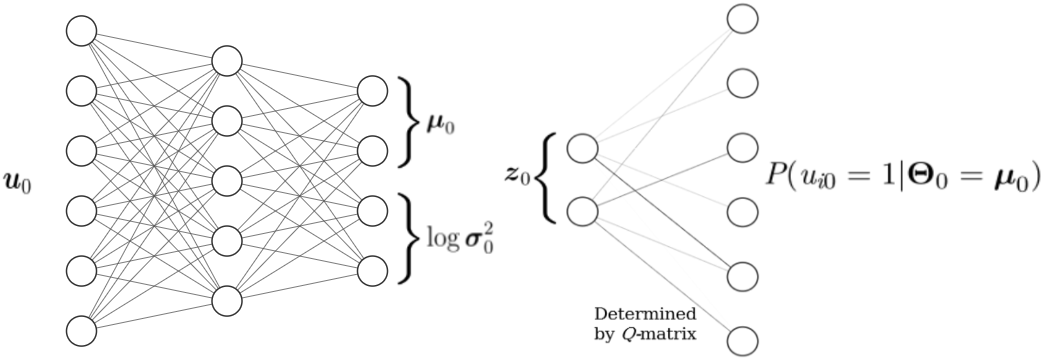
\includegraphics[width=0.95\textwidth]{../img/ml2p_vae_ind.png}
\end{center}
\begin{itemize}
  \item Trainable weights in decoder are item parameter estimates
  \item Feed responses $\vect u_0$ through encoder to obtain ability estimates $\vect \Theta_0 = \vect \mu_0$
\end{itemize}
\end{frame}

\begin{frame}{Advantages of ML2P-VAE Approach}
  For the IRT application:
  \begin{itemize}
    \item No trouble for high-dimensional $\vect \Theta$
    \item Doesn't directly optimize $\vect \Theta$
      \begin{itemize}
        \item Large number of students isn't a computational burden
      \end{itemize}
    \item Learning a \textit{function} that maps responses to latent abilities
      \begin{itemize}
        \item Encoder: $\vect u_0 \mapsto \vect \Theta_0$
      \end{itemize}
  \end{itemize}
  \onslide<2->{
  In the machine learning field:
  \begin{itemize}
    \item Ability to interpret a hidden neural layer
    \item Less abstract encoded latent space
    \item Explainable trainable parameters in decoder
  \end{itemize}
}%TODO: clean this slide up
\onslide<3->{Method originally presented at the International Joint Conference on Neural Networks (IJCNN) 2019}
\end{frame}

%TODO -- maybe include IJCNN results, but only if there is plenty of room

%\begin{frame}{ML2P-VAE Results}
%  \begin{itemize}
%    \item Simulated 28 item assessment with 3 latent skills and pre-determined $Q$-matrix 
%    \begin{itemize}
%      \item Discrimination and difficulty parameters randomly chosen 
%    \end{itemize}
%    \item $N$ subjects with latent skills drawn from $N(0,I)$
%    \item<2-> For each student $j$:
%    \begin{itemize}
%      \item<2-> For each item, calculate probability of success $P_{ij}$ from ML2P model
%      \item<2-> Sample from these probabilities to generate response set $U_j = (u_{j,1},...u_{j,28})$
%    \end{itemize}
%  \end{itemize}
%\end{frame}

%\begin{frame}{ML2P-VAE Results}
%\begin{center}
%\scriptsize
%
%Relative Error\\
%\begin{tabular}{ccccc}
%% \hline
%% &&&&\\
%\hline
%Size  & $a_1$ & $a_2$ & $a_3$ & $b$ \\
%\hline
%500   & 0.779 & 0.699 & 0.759 & 1.188 \\
%5,000 & 0.539 & 0.281 & 0.585 & 1.673 \\
%10,000  &0.284  & 0.159 & 0.264 & 1.894 \\
%\hline
%\end{tabular}
%
%\vspace{.5cm}
%
%Root Mean Square Error\\
%\begin{tabular}{ccccc}
%% \hline
%% &&&&\\
%\hline
%Size  & $a_1$ & $a_2$ & $a_3$ & $b$   \\
%\hline
%500   & 0.976 & 0.931 & 0.850 & 1.038 \\
%5,000 & 0.587 & 0.823 & 0.414 & 1.494 \\
%10,000  & 0.322 & 0.346 & 0.264 & 1.670 \\
%\hline
%\end{tabular}
%
%\vspace{.5cm}
%
%Correlation\\
%\begin{tabular}{ccccc}
%% \hline
%% &&&&\\
%\hline
%Size  & $a_1$ & $a_2$ & $a_3$ & $b$ \\
%\hline
%500   & 0.457 & 0.547 & 0.381 & 0.987 \\
%5000  & 0.779 & 0.710 & 0.990 & 0.982 \\
%10000   & 0.924 & 0.920 & 0.986 & 0.990 \\
%\hline
%\end{tabular}
%\end{center}
%\end{frame}
%
%\begin{frame}{ML2P-VAE Results}
%\begin{figure}[h!]
%\minipage{0.45\textwidth}
%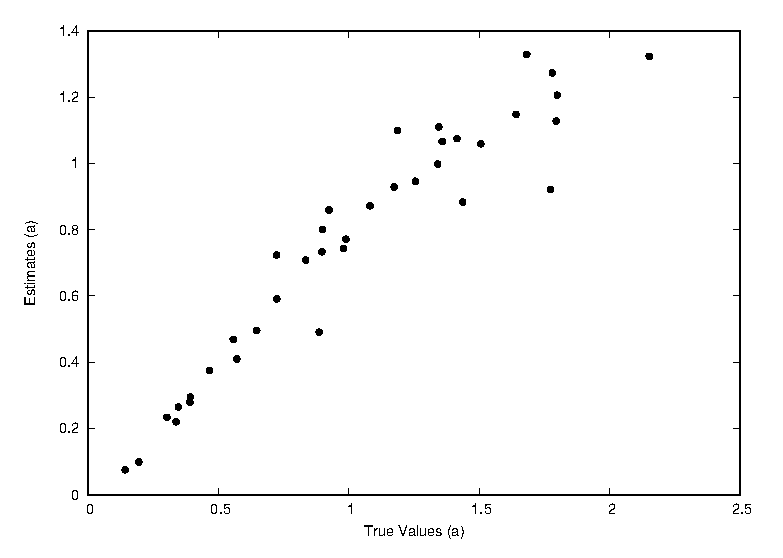
\includegraphics[width=\textwidth]{../img/ijcnn_results/10k_a.eps}
%\endminipage\hfill
%\minipage{0.45\textwidth}
%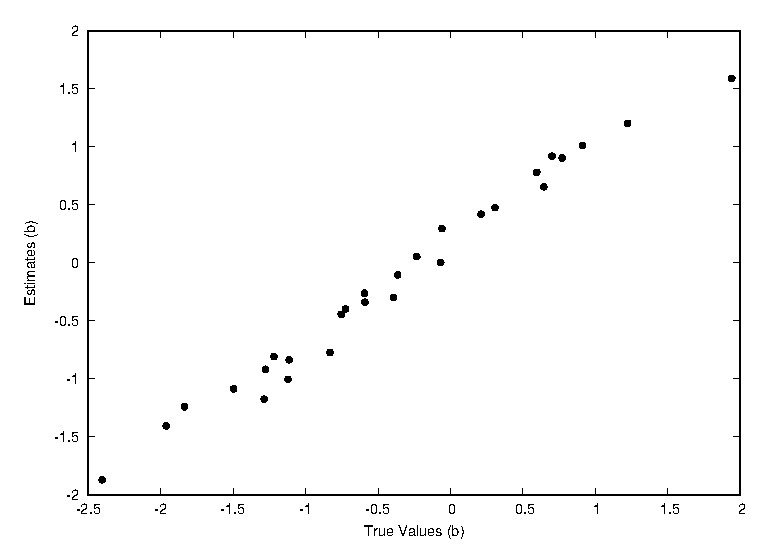
\includegraphics[width=\textwidth]{../img/ijcnn_results/10k_b.eps}
%\endminipage\hfill
%% \caption{Autoencoder and VAE discrimination parameter ($a_{ji}$) recovery.}
%% \label{fig:a_corr}
%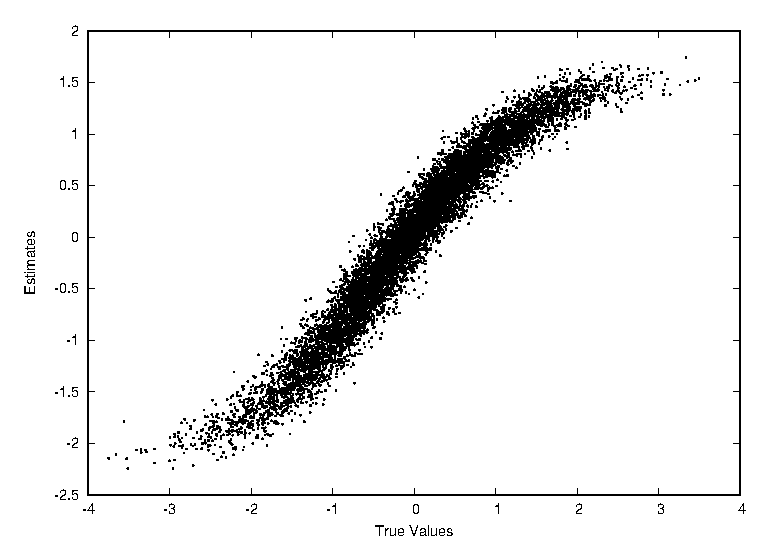
\includegraphics[width=.45\textwidth]{../img/ijcnn_results/10k_t1_scaled.eps}
%% \caption{test caption}
%% \label{f}
%\end{figure}
%\end{frame}


\subsection{Why use a \textit{Variational} Autoencoder?}

\begin{frame}{VAE vs AE Comparison}
  TODO: clean up and be better %TODO
\begin{itemize}
  \item Guo, Cutumisu, and Cui proposed using AE in skill estimation %TODO citation
  \item Directly compare neural networks in ML2P application
  \begin{itemize}
    \item Item parameter recovery
    \item Skill estimation
  \end{itemize}
\item<2-> How useful is prior $p(\vect \Theta)$?
\item<2-> What is the effect of the KL-Divergence term in the loss function?
\end{itemize}
\onslide<3->{Results presented at Artificial Intelligence in Education (AIED) 2019}
\end{frame}

%%%% probably don't want these tables
% \begin{frame}{VAE vs AE Comparison}
% \begin{table}[h]
%     \centering
%     \begin{tabular}{ccccc}
% \hline
% Model & $\theta_1$ & $\theta_2$ & $\theta_3$ & Statistic \\
% \hline
% AE &  7.425 & 3.107 & 16.260 & AVRB \\
% VAE   & 1.844 & 1.713 & 4.009 &  \\
% \hline
% AE & 1.788 & 1.523 & 1.746 & RMSE \\
% VAE   & 0.664 & 0.760 & 0.646 & \\
% \hline
% AE & 0.970 & 0.937 & 0.971 & CORR \\
% VAE   & 0.965 & 0.940 & 0.969 & \\
% \hline
%     \end{tabular}
%     \caption{Statistics for latent trait prediction with data size $n=10,000$.}
%     \label{tab:theta_stats}
% \end{table}
% \end{frame}

\begin{frame}{VAE vs AE Comparison}
\begin{figure}[h!]
\minipage{0.4\textwidth}
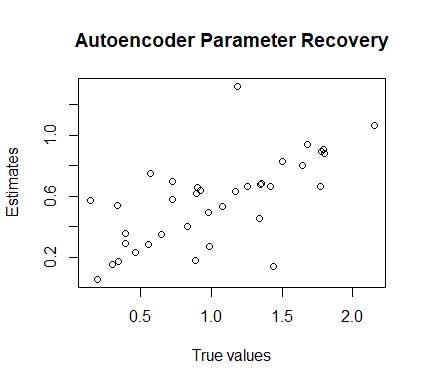
\includegraphics[width=.9\textwidth]{../img/aied_results/ae_a_corr.png}
\endminipage\hfill
\minipage{0.4\textwidth}
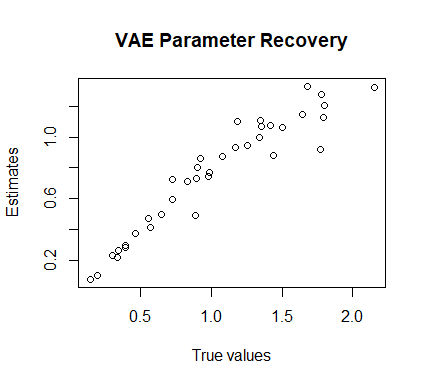
\includegraphics[width=.9\textwidth]{../img/aied_results/vae_a_corr.png}
\endminipage\hfill
\minipage{.2\textwidth}
{\footnotesize Discrimination \\ parameters $a_{ik}$}
\endminipage\hfill
\minipage{0.4\textwidth}
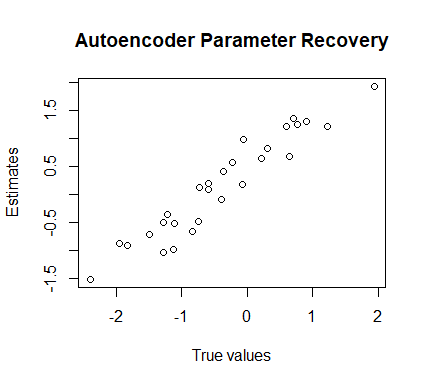
\includegraphics[width=.9\textwidth]{../img/aied_results/ae_b_corr.png}
\endminipage\hfill
\minipage{0.4\textwidth}
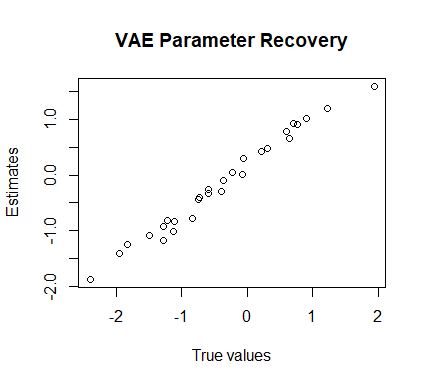
\includegraphics[width=.9\textwidth]{../img/aied_results/vae_b_corr.png}
\endminipage\hfill
\minipage{.2\textwidth}
{\footnotesize Difficulty \\ parameters $b_i$}
\endminipage\hfill
\end{figure}
\end{frame}

\begin{frame}{VAE vs AE Comparison}
\begin{figure}
\minipage{0.39\textwidth}
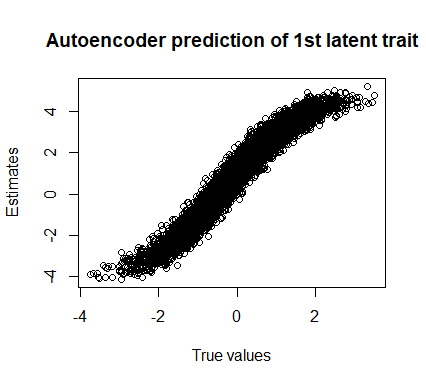
\includegraphics[width=\textwidth]{../img/aied_results/ae_theta1_corr.png}
\endminipage\hfill
\minipage{0.39\textwidth}
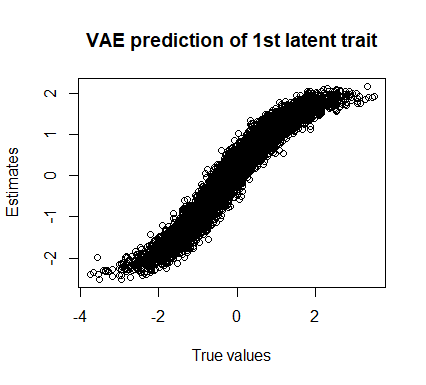
\includegraphics[width=\textwidth]{../img/aied_results/vae_theta1_corr.png}
\endminipage\hfill
\end{figure}
\begin{itemize}
  \item Similar skill estimate correlation, but on different scale %TODO: clean this up
  \item VAE much more accurate parameter recovery
\end{itemize}
\end{frame}


\subsection{Generalizing to Correlated Latent Traits}

\begin{frame}{Correlated Latent Traits in IRT}
\begin{itemize}
  \item In real applications, independent skills are not realistic: $\vect \Theta \sim \mathcal{N}(\vect \mu, \Sigma)$, not $\mathcal{N}(0,I)$.
  \begin{itemize}
    \item Example: students who are good at addition are also good at subtraction
  \end{itemize}
  \item<2-> Covariance matrix is symmetric, positive definite matrix
  \[\Sigma = \begin{bmatrix}
  \sigma_1^2 & c_{12} & \cdots & c_{1k} \\
  c_{21} & \sigma_2^2 & \cdots & c_{2k} \\
  \vdots & & \ddots & \vdots \\
  c_{k1} & \cdots & c_{k(k-1)} & \sigma_k^2
  \end{bmatrix}\]
  \item<2-> With variances $\sigma_i^2$ and covariances $c_{ij} = c_{ji}$
\end{itemize}
\end{frame}

\begin{frame}{Correlated Latent Code in VAE}
\begin{itemize}
  \item In most VAE applications, it is convenient to assume latent code $\vect z$ is \textit{independent}
    \begin{itemize}
      \item Forces each dimension of $\vect z$ to measure different features
      \item $\vect z$ is \textit{abstract}, with \textbf{no real-world understanding}
    \end{itemize}
  \item<2-> For ML2P-VAE, we know that latent code $\vect z$ approximates latent traits $\vect \Theta$
    \begin{itemize}
      \item<2-> We may have \textbf{domain knowledge} of the distribution of $\vect \Theta$
    \end{itemize}
\end{itemize}
\end{frame}

\begin{frame}{KL-Divergence for Multivariate Gaussians}
\begin{itemize}
  \item KL-Divergence between two $K$-dimensional multivariate Gaussian distributions:
\begin{align*}
&\mathcal{D}_{KL}\left[\mathcal{N}(\vect\mu_0, \Sigma_0) || \mathcal{N}(\vect\mu_1, \Sigma_1)\right] = \\
&\frac{1}{2} \left(\tr(\Sigma_1^{-1} \Sigma_0) + (\vect\mu_1 - \vect\mu_0)^T \Sigma_1^{-1} (\vect\mu_1 - \vect\mu_0) - K + \ln\left(\frac{\det \Sigma_1}{\det \Sigma_0} \right) \right)
\end{align*}
  \item<2-> When fitting a VAE, $\mathcal{N}(\vect\mu_1, \Sigma_1)$ is assumed to be known, so $\vect\mu_1$ and $\Sigma_1$ are constant
  \item<2-> $\vect\mu_0$ and $\Sigma_0$ obtained from feeding one sample through the encoder
\end{itemize}
\end{frame}

% \begin{frame}{Full Covariance Matrix in VAE}
% picture of full covariance VAE architecture
% \[\mu_0 = (m_1, m_2)^T\]
% \[L_0 = \begin{bmatrix}
% a_{11} & 0 \\ a_{21} & a_{22}
% \end{bmatrix}\]
% \end{frame}

\begin{frame}{Implementation Requirements for Correlated VAE}
\begin{enumerate}
  \item KL Divergence calculation uses $\vect\mu_0$, $\Sigma_0$, and $\ln\det \Sigma_0$ 
    \begin{itemize}
      \item<2-> Require $\det \Sigma_0 > 0$ for \underline{any} input $\vect u_0$
      \item<2-> $\Sigma_0$ is a function of the input $\vect u_0$ and every encoder weight 
    \end{itemize}
  \item Sample from a multivariate Gaussian $\mathcal{N}(\vect\mu_0, \Sigma_0)$:
  \begin{itemize}
    \item<3-> Find a matrix $G$ such that $G G^T = \Sigma_0$
    \item<3-> Sample $\vect\e = (\e_1,...,\e_k)^T$ with each $\e_i \sim \mathcal{N}(0,1)$
    \item<3-> Generate sample $\vect z_0 = \vect\mu_0 + G\vect\e$
  \end{itemize}
\end{enumerate}
\end{frame}

\begin{frame}{Correlated VAE Implementation}
\begin{itemize}
  \item Architecture: Encoder outputs $K + K(K+1)/2$ nodes
  \begin{itemize}
    \item $K$ nodes for $\vect\mu_0$, and $K(K+1)/2$ nodes for $L_0$ lower triangular
  \end{itemize}
  \item<2-> Sampling: Calculate $G_0 = e^{L_0}$ 
  \begin{itemize}
    \item<2-> Note $G_0$ is lower triangular, nonsingular
    \item<2-> Send sample $\vect z = \vect \mu_0 + G_0\vect\e$ through decoder
  \end{itemize}
  \item<3-> KL Divergence: Calculate $\Sigma_0 = G_0 G_0^T$
  \begin{itemize}
%    \item<3-> Note that
%  \begin{align*}
%  \det\Sigma_0 &= \det (e^{L_0} (e^{L_0})^T) = \det e^{L_0} \cdot \det (e^{L_0})^T \\
%  &= e^{\tr {L_0}} \cdot e^{\tr {L_0}^T} = \left(e^{\tr {L_0}}\right)^2 \\
%  &> 0
%  \end{align*}
\item<4-> Claim: $\Sigma_0$ is has positive determinant and is symmetric positive definite
  \end{itemize}
\end{itemize}
\end{frame}

\begin{frame}{Correlated VAE Implementation}
  \begin{theorem}
    \small
    Let $L_0$ be any lower triangular matrix. Then $\Sigma_0 = e^{L_0}\cdot \left(e^{L_0}\right)^\top$ is symmetric, positive definite, and has positive determinant.
  \end{theorem}
\begin{proof}
\tiny
\onslide<2->{Consider the matrix exponential 
\[G_0 := e^{L_0} = \sum_{n=0}^\infty \frac{L_0^n}{n!} = I + L_0 + \frac{1}{2}L_0^2 + \cdots\]}
\onslide<3->{$G_0$ is lower triangular, since addition and multiplication preserve lower triangular. $G_0$ is also nonsingular: 
\[\det G_0 = \det e^{L_0} = e^{\tr L_0} \not = 0\]}
\onslide<4->{Set $\Sigma_0 := G_0 G_0^T$. Now for any nonzero $\vect y \in \R^k$,}
\onslide<5->{\[\langle \Sigma_0\vect y, \vect y \rangle = \vect y^T \Sigma_0 \vect y = \vect y^T G_0 G_0^T \vect y = \langle G_0^T \vect y, G_0^T \vect y \rangle = ||G_0^T\vect y||_2^2 > 0\]}
\onslide<6->{Further, \[\det \Sigma_0 = \det \left(G_0 G_0^\top \right) = \det G_0 \cdot \det G_0^\top = e^{\tr L_0} \cdot e^{\tr L_0} > 0\]}
\end{proof}
\end{frame}

\begin{frame}{VAE architecture for correlated latent traits}
  \begin{figure}
  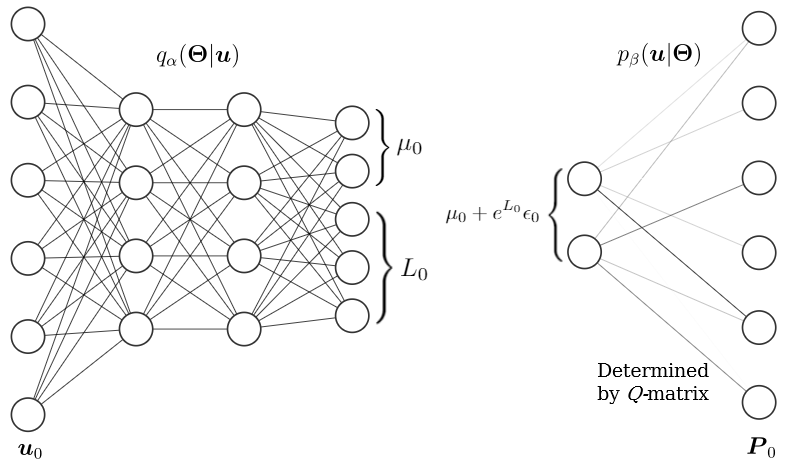
\includegraphics[width=.7\textwidth]{../img/ml2pvae_visual.png}
\caption*{Encoder structure for VAE learning $\mathcal{N}(\vect\mu,\Sigma)$}
\end{figure}
\end{frame}


\subsection{Method Comparison}

\begin{frame}{Comparison of ML2P-VAE vs Other Methods}
  \begin{itemize}
    \item MH-RM 
    \item MC-EM 
    \item QMC-EM
    \item ML2P-VAE$_{full}$ 
      \begin{itemize}
        \item Assume full knowledge of correlation matrix $\Sigma_1$
        \item Fit VAE with $\mathcal{N}(\vect 0, \Sigma_1)$
      \end{itemize}
    \item ML2P-VAE$_{est}$ 
      \begin{itemize}
        \item Unknown correlation matrix $\Sigma_1$ $\Rightarrow$ estimate it with $\tilde \Sigma_1$
        \item Fit VAE with $\mathcal{N}(\vect 0, \tilde \Sigma_1)$
      \end{itemize}
    \item ML2P-VAE$_{ind}$ 
      \begin{itemize}
        \item Unknown correlation matrix $\Sigma_1$ $\Rightarrow$ assume independent $\vect \Theta$
        \item Fit VAE with $\mathcal{N}(\vect 0, I)$
      \end{itemize}
  \end{itemize}
\end{frame}

\begin{frame}{Datasets}
  \begin{table}
    \centering
    \begin{tabular}{c|ccc}
      & Items & Skills & Students \\
      \hline
      ECPE & 28 & 3 & 2,922 \\ 
      Sim-6 & 50 & 6 & 20,000 \\
      Sim-20 & 200 & 20 & 50,000 \\
      Sim-4 & 27 & 4 & 3,000  
    \end{tabular}
  \end{table}
\end{frame}

\begin{frame}{Sim-6 Discrimination Parameter Estimates}
\begin{figure}[h]
\centering
    \begin{subfigure}{.32\textwidth}
      \centering
      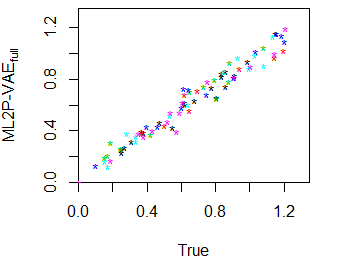
\includegraphics[width=.9\linewidth]{../img/ml_journal_results/6skills/vae_full_disc_6skills.png}
    \end{subfigure}
    \begin{subfigure}{.32\textwidth}
      \centering
      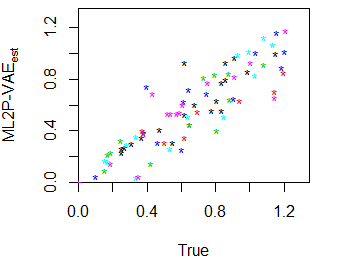
\includegraphics[width=.9\linewidth]{../img/ml_journal_results/6skills/vae_est_disc_6skills.png}
    \end{subfigure}
    \begin{subfigure}{.32\textwidth}
      \centering
      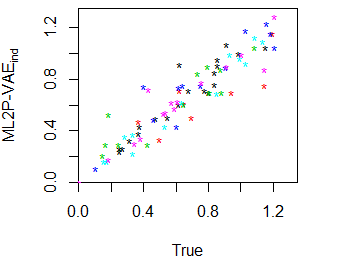
\includegraphics[width=.9\linewidth]{../img/ml_journal_results/6skills/vae_ind_disc_6skills.png}
    \end{subfigure}
    \begin{subfigure}{.32\textwidth}
      \centering
      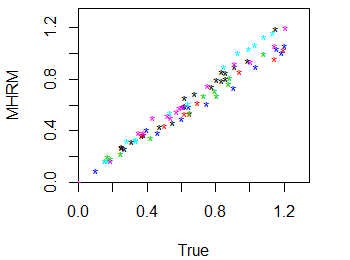
\includegraphics[width=.9\linewidth]{../img/ml_journal_results/6skills/mhrm_disc_6skills.png}
    \end{subfigure}
    \begin{subfigure}{.32\textwidth}
      \centering
      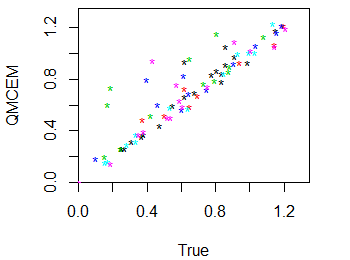
\includegraphics[width=.9\linewidth]{../img/ml_journal_results/6skills/qmcem_disc_6skills.png}
    \end{subfigure}
    \begin{subfigure}{.32\textwidth}
      \centering
      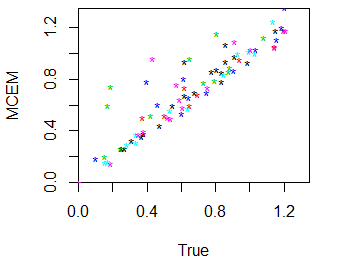
\includegraphics[width=.9\linewidth]{../img/ml_journal_results/6skills/mcem_disc_6skills.png}
    \end{subfigure}
    \caption{Correlation plots of discrimination parameter estimates for the Sim-6 dataset with 50 items and 6 latent traits. ML2P-VAE estimates are on the top row, and traditional method estimates are on the bottom row.}
    \label{fig:6skill_cor}
\end{figure}
\end{frame}

\begin{frame}{ECPE Parameter Estimates}
\begin{figure}[h]
\centering
    \begin{subfigure}{.32\textwidth}
      \centering
      \figuretitlesmall{Discrimination Parameters}
      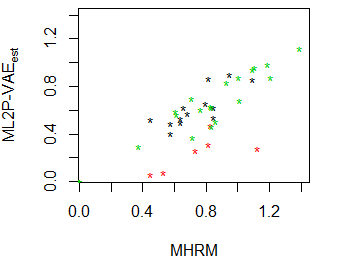
\includegraphics[width=.9\linewidth]{../img/ml_journal_results/ecpe/vae_est_disc_ecpe.png}
    \end{subfigure}
    \begin{subfigure}{.32\textwidth}
      \centering
      \figuretitlesmall{Difficulty Parameters}
      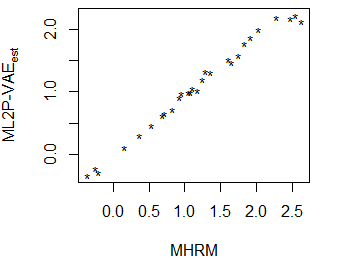
\includegraphics[width=.9\linewidth]{../img/ml_journal_results/ecpe/vae_est_diff_ecpe.png}
    \end{subfigure}
    \begin{subfigure}{.32\textwidth}
      \centering
      \figuretitlesmall{Ability Parameters}
      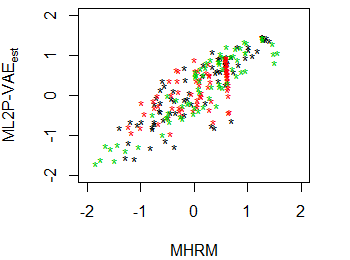
\includegraphics[width=.9\linewidth]{../img/ml_journal_results/ecpe/vae_est_theta_ecpe.png}
    \end{subfigure}
    \begin{subfigure}{.32\textwidth}
      \centering
      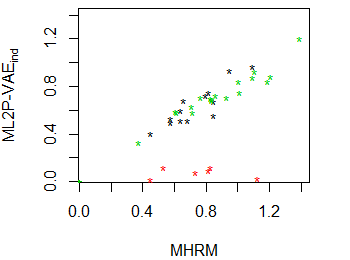
\includegraphics[width=.9\linewidth]{../img/ml_journal_results/ecpe/vae_ind_disc_ecpe.png}
    \end{subfigure}
    \begin{subfigure}{.32\textwidth}
      \centering
      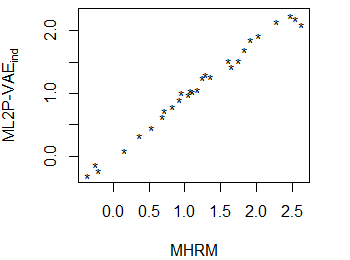
\includegraphics[width=.9\linewidth]{../img/ml_journal_results/ecpe/vae_ind_diff_ecpe.png}
    \end{subfigure}
    \begin{subfigure}{.32\textwidth}
      \centering
      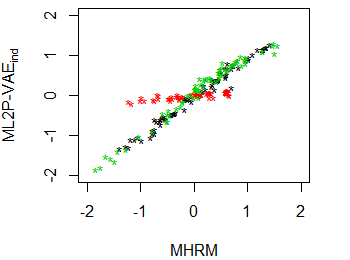
\includegraphics[width=.9\linewidth]{../img/ml_journal_results/ecpe/vae_ind_theta_ecpe.png}
    \end{subfigure}
    \caption{Estimates from ML2P-VAE methods plotted against ``accepted'' MHRM estimates from the ECPE dataset.}
    \label{fig:ecpe_cor}
\end{figure}


\end{frame}

\begin{frame}{Sim-20 Parameter Estimates}
\begin{figure}[h]
\centering
\figuretitle{Discrimination and Ability Parameter Estimates}\\
    \begin{subfigure}{.32\textwidth}
      \centering
      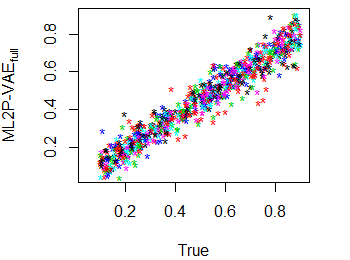
\includegraphics[width=.9\linewidth]{../img/ml_journal_results/20skills/vae_full_disc_20skills.png}
    \end{subfigure}
    \begin{subfigure}{.32\textwidth}
      \centering
      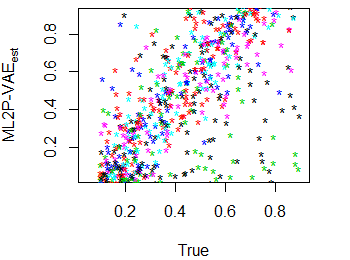
\includegraphics[width=.9\linewidth]{../img/ml_journal_results/20skills/vae_est_disc_20skills.png}
    \end{subfigure}
    \begin{subfigure}{.32\textwidth}
      \centering
      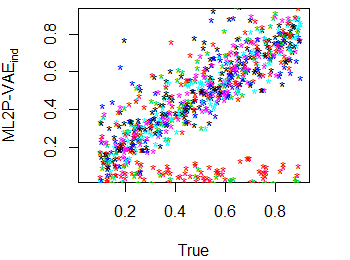
\includegraphics[width=.9\linewidth]{../img/ml_journal_results/20skills/vae_ind_disc_20skills.png}
    \end{subfigure}
    \begin{subfigure}{.32\textwidth}
      \centering
      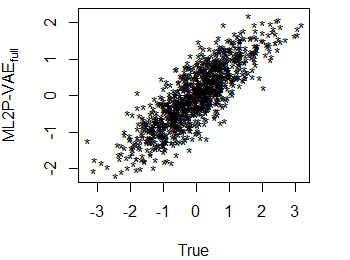
\includegraphics[width=.9\linewidth]{../img/ml_journal_results/20skills/vae_full_theta_20skills.png}
    \end{subfigure}
    \begin{subfigure}{.32\textwidth}
      \centering
      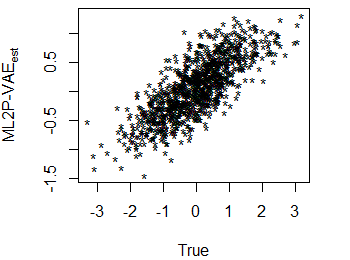
\includegraphics[width=.9\linewidth]{../img/ml_journal_results/20skills/vae_est_theta_20skills.png}
    \end{subfigure}
    \begin{subfigure}{.32\textwidth}
      \centering
      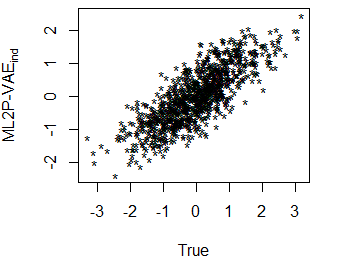
\includegraphics[width=.9\linewidth]{../img/ml_journal_results/20skills/vae_ind_theta_20skills.png}
    \end{subfigure}
    \caption{ML2P-VAE parameter estimates for Sim-20 with 200 items and 20 latent traits. The top row shows discrimination parameter correlation, and the bottom row shows ability parameter correlation.}
    \label{fig:20skill_cor}
\end{figure}


\end{frame}

\begin{frame}{Sim-4 Discrimination Parameter Estimates}
\begin{figure}[h]
\centering
\figuretitle{Discrimination Parameter Estimates}\\
    \begin{subfigure}{.32\textwidth}
      \centering
      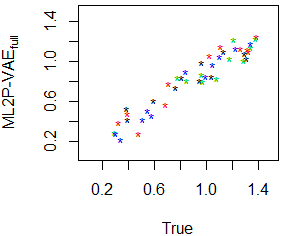
\includegraphics[width=.9\linewidth]{../img/ml_journal_results/4skills/vae_full_disc_4skills_cropped.png}
    \end{subfigure}
    \begin{subfigure}{.32\textwidth}
      \centering
      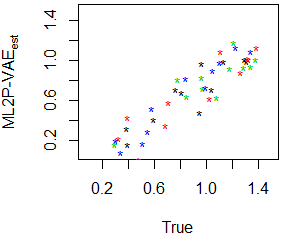
\includegraphics[width=.9\linewidth]{../img/ml_journal_results/4skills/vae_est_disc_4skills_cropped.png}
    \end{subfigure}
    \begin{subfigure}{.32\textwidth}
      \centering
      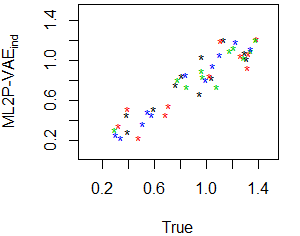
\includegraphics[width=.9\linewidth]{../img/ml_journal_results/4skills/vae_ind_disc_4skills_cropped.png}
    \end{subfigure}
    \begin{subfigure}{.32\textwidth}
      \centering
      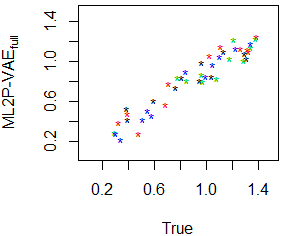
\includegraphics[width=.9\linewidth]{../img/ml_journal_results/4skills/vae_full_disc_4skills_cropped.png}
    \end{subfigure}
    \begin{subfigure}{.32\textwidth}
      \centering
      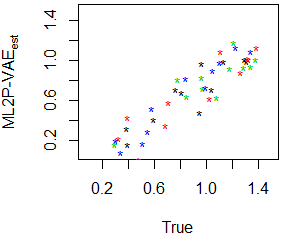
\includegraphics[width=.9\linewidth]{../img/ml_journal_results/4skills/vae_est_disc_4skills_cropped.png}
    \end{subfigure}
    \begin{subfigure}{.32\textwidth}
      \centering
      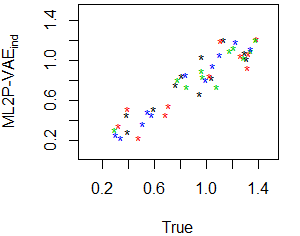
\includegraphics[width=.9\linewidth]{../img/ml_journal_results/4skills/vae_ind_disc_4skills_cropped.png}
    \end{subfigure}
    \caption{Discrimination parameter estimates for Sim-4 with 27 items and 4 latent skills. The top row shows estimates from ML2P-VAE methods, and the bottom row gives estimates yielded by traditional methods.}
    \label{fig:4skills_disc}
\end{figure}


\end{frame}

\begin{frame}{Correlated ML2P-VAE Results}
  %TODO maybe put into two slides?
  \tiny
\begin{tabular}{c|c|ccc|ccc|ccc|c}
  \hline
    Data Set & Method & $\vect a$.RMSE & $\vect a$.BIAS & $\vect a$.COR & $\vect b$.RMSE & $\vect b$.BIAS & $\vect b$.COR &  $\vect \Theta$.RMSE & $\vect \Theta$.BIAS & $\vect \Theta$.COR & Runtime \\
    \hline
& MHRM & 0.0693 & 0.0319  & 0.9986   & 0.0256 & -0.0021 & 0.9999  & 0.714  & -0.0033  & 0.7006 & 1110s \\ 
(i)& QMCEM & 0.149 & -0.067 & 0.9939 & 0.0376 & -0.002 & 0.9998 & 0.7206 & 0.0023 & 0.6939 & 322s\\
6 abilities& MCEM & 0.1497 & -0.0633 &  0.9936 &  0.0383 & 0.0035 & 0.9997 &  0.7206 & -0.0016 & 0.6938 & 1009s\\
Sim-6& ML2P-VAE$_{full}$ & 0.0705 &  0.0255  & 0.9985   & 0.0471 & -0.0079 & 0.9996  & 0.6649   & -0.0178  & 0.7476 & 343s\\
& ML2P-VAE$_{est}$ & 0.1803 & 0.0871  & 0.9891 &  0.064 & -0.0131 & 0.9993  & 0.7109 &  0.0772  & 0.7082 & 364s \\
& ML2P-VAE$_{ind}$ & 0.1218 & -0.0004 & 0.9944   & 0.0597 & -0.0145 & 0.9994  & 0.7222 &  0.0316  & 0.6928 & 252s\\
\hline 
& MHRM* & 0* & 0*&  1* &  0* &  0* &  1* & 0* & 0* &  1* & 162s \\
(ii)& QMCEM & 0.0159  & 0.0035 & 0.9999 & 0.0067  & -0.0005 & 1   & 0.0111 & 0.0007 & 0.9999 & 33s\\
3 abilities & MCEM & 0.0228 & 0.0148 & 0.9998 & 0.0064  & -0.0008 & 1   & 0.0132 & 0.0026 & 0.9998 & 192s \\
ECPE & ML2P-VAE$_{full}$ & N/A & N/A & N/A & N/A & N/A & N/A & N/A & N/A & N/A & N/A  \\
& ML2P-VAE$_{est}$ & 0.2794 & 0.2152 & 0.9713 & 0.148 & 0.0951  & 0.993 & 0.443 & -0.0628 & 0.8237 & 61s  \\
& ML2P-VAE$_{ind}$ & 0.3208 & 0.2184 & 0.9504 & 0.154 & 0.0872  & 0.9932  & 0.3063 & 0.01 & 0.9017 & 49s \\
\hline
& MHRM & N/A & N/A & N/A & N/A & N/A & N/A & N/A & N/A & N/A & N/A  \\
(iii)& QMCEM & N/A & N/A & N/A & N/A & N/A & N/A & N/A & N/A & N/A & N/A \\
20 abilities & MCEM & N/A & N/A & N/A & N/A & N/A & N/A & N/A & N/A & N/A & N/A  \\
Sim-20 & ML2P-VAE$_{full}$ & 0.078 &  0.0473  & 0.9983  & 0.0608 &  0.0054  & 0.9996  & 0.6145 &  0.0065  & 0.7893 & 1292s \\
& ML2P-VAE$_{est}$ & 0.2992  & -0.1304  & 0.9822  & 0.1655 &  0.1215  & 0.9987  & 0.7364   & -0.0276  & 0.7257 & 961s \\
& ML2P-VAE$_{ind}$ & 0.2043 &   0.0592  & 0.9792  & 0.0958   & -0.0029  & 0.9992  & 0.7054 &  0.0747  & 0.7135 & 850s \\
\hline 
        & MHRM & 0.0953 & -0.0158	&	0.9966 & 0.0614 & -0.0101 &	0.9988 & 0.6325	& 0.0118	& 0.7697 & 94s \\
        (iv)& QMCEM & 0.0938 & -0.0160	&	0.9967 & 0.0614 & -0.0179 &	0.9989 & 0.6326	& 0.0154	& 0.7696 & 29s \\
        4 abilities & MCEM & 0.0951 & -0.0138	&	0.9966 & 0.0644 & -0.0199 &	0.9987 & 0.6326	& 0.0150	& 0.7696 & 196s \\
       Sim-4 & ML2P-VAE$_{full}$ & 0.1326 & 0.0780		&	0.9960 & 0.0872 & -0.0311 &	0.9978 & 0.6384	& 0.0210	& 0.7648 & 37s \\
        & ML2P-VAE$_{est}$ & 0.2526 & 0.2106		&	0.9883 & 0.1035 & -0.0337 &	0.9980 & 0.6897	& -0.0256 	& 0.7182 & 38s \\
        & ML2P-VAE$_{ind}$ & 0.1658 & 0.1099		&	0.9939 & 0.0944 & -0.0254 &	0.9976 & 0.6474	& -0.0397	& 0.7579 & 30s \\

\hline
\end{tabular}
\end{frame}

\begin{frame}{Scalability of ML2P-VAE}
\begin{figure}[h]
\centering
    \begin{subfigure}{.47\textwidth}
      \centering
      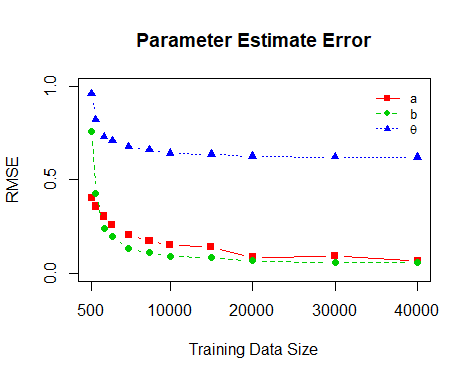
\includegraphics[width=\linewidth]{../img/ml_journal_results/vae_full_train_size_error.png}
    \end{subfigure}
    \begin{subfigure}{.47\textwidth}
      \centering
      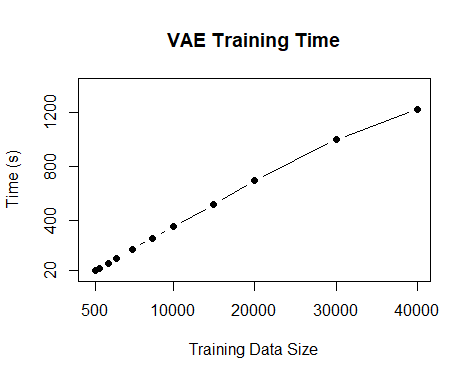
\includegraphics[width=\linewidth]{../img/ml_journal_results/vae_full_train_size_time.png}
    \end{subfigure}
    \caption{Performance of ML2P-VAE$_{full}$ on data set (iii) when trained on data sets of increasing size. The left plot gives the test RMSE after using different sizes of training data, and the right plot shows the time required to train the neural network.}
    \label{fig:train_size}
\end{figure}


\end{frame}

\subsection{ML2Pvae R Package}
\begin{frame}{ML2Pvae Package in R}
\begin{itemize}
  \item Software package on CRAN for easy implementation of ML2P-VAE methods
    \begin{itemize}
      \item For IRT researchers -- requires no knowledge of neural networks or TensorFlow
    \end{itemize}
  \item<2-> Package functions:
  \begin{itemize}
    \item<2-> Construct ML2P-VAE model to desired architecture
      \begin{itemize}
        \item<2-> Option for independent latent traits or full covariance matrix
      \end{itemize}
    \item<2-> Wrapper function to train neural network
    \item<2-> Simple functions to obtain parameter estimates after training
  \end{itemize}
\end{itemize}
\end{frame}


\section{Knowledge Tracing}

\begin{frame}{Bayesian Knowledge Tracing}
  TODO: background/motivation of KT
\end{frame}

\subsection{Temporal Neural Networks}
\begin{frame}{RNN / LSTM}
  RNN, LSTM 
\end{frame}

\begin{frame}{Attention-based networks}
  Transformer / Attention
\end{frame}

\subsection{Deep Knowledge Tracing Methods}
\begin{frame}{Deep Knowledge Tracing}
  DKT
\end{frame}

\begin{frame}{SAKT}
  SAKT
\end{frame}

\begin{frame}{Other methods}
  might want to mention DKVMN or PFA
\end{frame}

\subsection{Incorporating IRT into Knowledge Tracing}
\begin{frame}{Do deep models actually ``trace'' knowledge?}
  motivation
\end{frame}

\begin{frame}{IRT-inspired Knowledge Tracing}
  method description
\end{frame}

\begin{frame}{IRT-inspired Knowledge Tracing}
  image of architecture
\end{frame}

\subsection{Results}
\begin{frame}{Datasets}
  datasets
\end{frame}

\begin{frame}{Results}
  Table and theta trace plot
\end{frame}

\begin{frame}{Recovery of IRT parameters}
  disc and theta recovery plots
\end{frame}

\begin{frame}{Learning a $Q$-matrix}
  cor heatmap and clustering
\end{frame}


\section{Future Work}

\subsection{ML2P-VAE}
\begin{frame}{Extending ML2P-VAE to other IRT models}
  3PL and Samejima
\end{frame}

\begin{frame}{Other application areas}
  BDI and personality questionnaires
\end{frame}

\subsection{IRT-inspired Knowledge Tracing}
\begin{frame}{Utilizing more domain knowledge}
  use Q matrix in attn calculation
  missing responses with embedding of interactions
\end{frame}


\section{Conclusions}
\begin{frame}{Summary}
  
\end{frame}

\begin{frame}{Summary}
  
\end{frame}

\section*{Acknowledgements}
\begin{frame}{Thank you!}
  
\end{frame}

\section{}
\begin{frame}{References}
    TODO: choose citations in the right way %TODO
\begin{thebibliography}{2}
\tiny

\bibitem{thissen} Wainer and Thissen, D. ``Test Scoring''. Erlbaum Associates, Publishers, 2001.

\bibitem{dasilva} da Silva, Liu, Huggins-Manley, Bazan. ``Incorporating the Q-matrix into Multidimensional Item Response Models.'' Journal of Educational and Psychological Measurement, 2018.

\bibitem{baker} Baker and Kim. ``Item Response Theory: Parameter Estimation Techniques''. CRC Press, 2004.

\bibitem{bock} Bock and Aitken. ``Marginal Maximum Likelihood Estimation of Item Parameters: Application of an EM Algorithm''. Psychometrika, 1981.

\bibitem{nielsen} Nielsen, Michael. ``Neural Networks and Deep Learning''. Determination Press, 2015.

\bibitem{ijcnn} Curi, Converse, Hajewski, Oliveira. ``Interpretable Variational Autoencoders for Cognitive Models.'' In Proceddings of the International Joint Conference on Neural Networks (IJCNN), 2019.

\bibitem{guo} Q. Guo, M. Cutumisu, and Y. Cui. ``A Neural Network Approach to Estimate Student Skill Mastery in Cognitive Diagnostic Assessments''. In: 10th International Conference on Educational Data Mining. 2017.

\bibitem{aied} Converse, Curi, Oliveira. ``Autoencoders for Educational Assessment.'' In Proceedings of the Conference on Artifical Intelligence in Education (AIED), 2019.

\bibitem{fsdm} Converse, Curi, Oliveira, and Arnold. ``Variational Autoencoders for Baseball Player Evaluation.'' In Proceedings of the Fuzzy Systems and Data Mining Conference (FSDM), 2019.  


\end{thebibliography}
\end{frame}

\begin{frame}
  \titlepage
\end{frame}

\end{document}
